\documentclass[11pt]{article}

% ---------------------------------------------------------------------------
% PAC-Bayesian Generalization Bounds for Weight-Decomposed Low-Rank Adaptation
% 6-page theory report: full proofs retained; Gibbs section removed; experiments
% trimmed to the verification of Theorems 3.10 (identity) and 3.4 (KL bracket).
% Compile:  pdflatex main.tex   (run twice for references)
% ---------------------------------------------------------------------------

\usepackage[margin=1in]{geometry}
\usepackage{amsmath,amssymb,amsthm}
\usepackage{graphicx}
\usepackage{booktabs}
\usepackage{caption}
\usepackage[colorlinks=true,linkcolor=blue,citecolor=blue,urlcolor=blue]{hyperref}
\usepackage{enumitem}

\graphicspath{{figures/}}

% compact spacing to fit 6 pages
\setlength{\parskip}{2pt}
\captionsetup{font=small}

\newtheorem{theorem}{Theorem}
\newtheorem{lemma}{Lemma}
\newtheorem{remark}{Remark}
\newtheorem{assumption}{Assumption}

\newcommand{\KL}{\mathrm{KL}}
\newcommand{\vMF}{\mathrm{vMF}}
\newcommand{\Risk}{R}
\newcommand{\eRisk}{\hat{R}}
\newcommand{\Cdir}{C_{\mathrm{dir}}}
\newcommand{\Sd}{\mathbb{S}^{d-1}}
\newcommand{\Thetaglob}{\Theta_{\mathrm{global}}}
\newcommand{\E}{\mathbb{E}}
\newcommand{\R}{\mathbb{R}}

\title{\textbf{PAC-Bayesian Generalization Bounds for\\
Weight-Decomposed Low-Rank Adaptation}}
\author{Stephen Zhang \and Varun Prakash \and Soham [Surname]}
\date{\today}

\begin{document}
\maketitle
\vspace{-1.5em}

\begin{abstract}
\small
Parameter-efficient fine-tuning (PEFT) methods such as DoRA and MAP decompose weight
updates into magnitude and directional components, yet their generalization behavior
is poorly understood. We give a PAC-Bayesian analysis of weight-decomposed adaptation
using von Mises--Fisher (vMF) priors on the hypersphere, yielding closed-form KL
complexity terms in the angular deviations between pretrained and fine-tuned
directions. We prove non-asymptotic KL bounds valid beyond the high-concentration
regime, and a comparison theorem showing that column-wise methods (DoRA)
\emph{sum} directional complexity over local angles while global methods (MAP)
\emph{average} it into a single rotation---so DoRA is favored under sparse, localized
updates and MAP under globally aligned ones. We then validate the two geometric
theorems empirically: fine-tuning RoBERTa-base under LoRA/DoRA/MAP and measuring
per-column angles over $2592$ weight matrices, the sum-vs-average identity holds to
machine precision (and with $R^2{=}0.995$ in its measured form), the non-asymptotic
KL bracket holds with zero violations, and the non-asymptotic correction tightens the
directional KL by $77$--$307\times$ at transformer dimensions.
\end{abstract}

\section{Introduction}
Large pretrained models are adapted to downstream tasks via parameter-efficient
fine-tuning (PEFT), which modifies a small subset of parameters. Recent methods such
as DoRA~\cite{dora} and MAP~\cite{map} adopt a \emph{weight-decomposition} view,
representing parameters by magnitude and direction. DoRA updates each column of a
weight matrix independently (column-wise rotations); MAP rotates the entire flattened
matrix as one vector. There is no theory explaining when one should generalize better
than the other.

We close this gap with a PAC-Bayesian analysis. Modeling directional updates with vMF
distributions on the hypersphere yields generalization bounds depending explicitly on
angular deviations, giving a notion of \emph{directional complexity}. Our
contributions: (i) non-asymptotic vMF KL bounds (Theorems~\ref{thm:nonasym},
\ref{thm:dora-bound}, \ref{thm:map-bound}); (ii) a comparison theorem
(Theorem~\ref{thm:comparison}) with a sharp local-vs-global characterization; and
(iii) an empirical verification of the two geometric theorems on RoBERTa-base.

\section{Background}
\textbf{PEFT.} LoRA~\cite{lora} writes $\Delta W=BA$ with $B\in\R^{d\times r}$,
$A\in\R^{r\times d}$, $r\ll d$. DoRA~\cite{dora} decomposes each column
$w_j=m_j u_j$, $m_j\in\R_+$, $u_j\in\Sd$, updating the direction via LoRA and the
magnitude directly. MAP~\cite{map} flattens $W\in\R^{d\times d}$ to $w\in\R^{d^2}$ and
writes $w'=\alpha\hat w+\beta\widehat{\Delta w}$ with unit $\hat w,\widehat{\Delta w}$
and learnable $\alpha,\beta$.

\textbf{PAC-Bayes.} Bounds~\cite{mcallester,catoni} control the risk of a randomized
predictor through $\KL(Q\|P)$ between posterior $Q$ and data-free prior $P$.

\textbf{vMF.} $\vMF(\mu,\kappa)$ on $\Sd$ has density
$p(x\mid\mu,\kappa)=C_d(\kappa)\exp(\kappa\mu^\top x)$ with mean resultant length
$A_d(\kappa)=I_{d/2}(\kappa)/I_{d/2-1}(\kappa)\in[0,1)$, strictly increasing in
$\kappa$; $\kappa\to\infty$ concentrates at $\mu$, $\kappa=0$ is uniform.

\section{PAC-Bayesian Analysis of Weight-Decomposed Adaptation}

\subsection{Setup}
Let $P$ be a data-free prior and $Q$ a posterior on a sample $S\sim\mathcal{D}^n$,
loss $\ell\in[0,1]$. Write $\Risk(Q)=\E_{h\sim Q}\E_z[\ell]$ and
$\eRisk(Q)=\E_{h\sim Q}\frac1n\sum_i\ell(h,z_i)$.

\begin{theorem}[McAllester~\cite{mcallester}]\label{thm:mcallester}
For any $\delta\in(0,1)$, w.p.\ $\ge1-\delta$, for all $Q$:
$\Risk(Q)\le\eRisk(Q)+\sqrt{(\KL(Q\|P)+\ln\tfrac{2\sqrt n}{\delta})/2n}.$
\end{theorem}
Bounding $\Risk(Q)$ thus reduces to bounding $\KL(Q\|P)$ under the structured
parameterizations of DoRA and MAP.

\subsection{Non-Asymptotic vMF KL Bounds}

\begin{lemma}[vMF KL, equal concentration]\label{lem:vmfkl}
For $Q_1=\vMF(\mu_1,\kappa)$, $Q_0=\vMF(\mu_0,\kappa)$ on $\Sd$,
$\KL(Q_1\|Q_0)=\kappa A_d(\kappa)(1-\mu_1^\top\mu_0).$
\end{lemma}
\begin{proof}
$\KL=\E_{Q_1}[\ln p(x\mid\mu_1,\kappa)-\ln p(x\mid\mu_0,\kappa)]
=\kappa(\mu_1-\mu_0)^\top\E_{Q_1}[x]$, since the normalizers $C_d(\kappa)$ cancel at
equal $\kappa$. The vMF mean is $\E_{Q_1}[x]=A_d(\kappa)\mu_1$ (App.~\ref{app:mean}),
so $\KL=\kappa A_d(\kappa)(\mu_1^\top\mu_1-\mu_1^\top\mu_0)=\kappa A_d(\kappa)(1-\mu_1^\top\mu_0)$.
\end{proof}

\begin{lemma}[Bounds on $A_d$]\label{lem:adbounds}
For all $\kappa>0,\,d\ge2$: $\ \kappa/(d+\kappa)\le A_d(\kappa)\le1.$
\end{lemma}
\begin{proof}
The upper bound is immediate: $A_d(\kappa)=\E_{\vMF(\mu,\kappa)}[\mu^\top x]\le1$ as
$\mu^\top x\le1$. The lower bound is the Amos Bessel-ratio inequality~\cite{amos}
$\tfrac{I_{d/2}(\kappa)}{I_{d/2-1}(\kappa)}\ge\tfrac{\kappa}{d/2+\sqrt{d^2/4+\kappa^2}}\ge\tfrac{\kappa}{d+\kappa}$,
the last step using $\sqrt{d^2/4+\kappa^2}\le d/2+\kappa$.
\end{proof}

\begin{theorem}[Non-asymptotic directional KL bracket]\label{thm:nonasym}
Under the column-wise (DoRA) decomposition with per-column vMF priors of
concentration $\kappa$ and angles $\theta_j$,
\[
\tfrac{\kappa^2}{d+\kappa}\textstyle\sum_{j=1}^d(1-\cos\theta_j)
\ \le\ C^{\mathrm{DoRA}}_{\mathrm{dir}}
\ \le\ \kappa\textstyle\sum_{j=1}^d(1-\cos\theta_j),
\]
and under the global (MAP) decomposition with angle $\Thetaglob$,
$\frac{\kappa^2}{k+\kappa}(1-\cos\Thetaglob)\le C^{\mathrm{MAP}}_{\mathrm{dir}}
\le\kappa(1-\cos\Thetaglob).$
\end{theorem}
\begin{proof}
By Lemma~\ref{lem:vmfkl}, $C^{\mathrm{DoRA}}_{\mathrm{dir}}=\sum_j\KL(Q_{\mathrm{dir},j}\|P_{\mathrm{dir},j})
=\kappa A_d(\kappa)\sum_j(1-\cos\theta_j)$. Substituting the two bounds on $A_d(\kappa)$
from Lemma~\ref{lem:adbounds} gives the bracket. The MAP case is identical with $d\!\to\!k$
and the sum replaced by the single global term.
\end{proof}

\begin{remark}
The bracket holds for all $\kappa>0$, removing any need for $\kappa\to\infty$. Since
$A_d(\kappa)\approx\kappa/d$ for $\kappa\ll d$, the exact KL sits near the lower bound,
and the asymptotic approximation ($A_d\!\equiv\!1$, the upper bound) overestimates the
directional KL by a factor $1/A_d(\kappa)$---verified empirically in
Section~\ref{sec:experiments}.
\end{remark}

\subsection{DoRA: Column-Wise Decomposition}
For $W\in\R^{d\times d}$ with $w_j=m_j u_j$, assume (A1) mean-field
$P=\prod_j P_j,\,Q=\prod_j Q_j$; (A2) independent magnitude/direction; (A3) Gaussian
magnitudes $\mathcal{N}(\cdot,\sigma^2)$; (A4) vMF directions with shared $\kappa$.
Then the KL factorizes:
\begin{equation}\label{eq:kldecomp}
\KL(Q\|P)=\sum_{j=1}^d\Big[\underbrace{\tfrac{(\hat m_j-m_{0,j})^2}{2\sigma^2}}_{\text{magnitude}}
+\underbrace{\kappa A_d(\kappa)(1-\cos\theta_j)}_{\text{direction}}\Big],
\end{equation}
with $\theta_j=\arccos(\hat\mu_j^\top\mu_{0,j})$. The first term is the standard
equal-variance Gaussian KL $(\hat m_j-m_{0,j})^2/2\sigma^2$; the second is
Lemma~\ref{lem:vmfkl}.

\begin{theorem}[PAC-Bayes bound, DoRA]\label{thm:dora-bound}
W.p.\ $\ge1-\delta$,
$\Risk(Q)\le\eRisk(Q)+\sqrt{\big(\sum_j[\frac{(\hat m_j-m_{0,j})^2}{2\sigma^2}
+\kappa A_d(\kappa)(1-\cos\theta_j)]+\ln\frac{2\sqrt n}{\delta}\big)/2n}.$
In the regime $\kappa\gg d,\ \theta_j\ll1$, $A_d(\kappa)\to1$ and $1-\cos\theta_j\to\theta_j^2/2$,
giving $\KL\approx\sum_j[\frac{(\hat m_j-m_{0,j})^2}{2\sigma^2}+\frac\kappa2\theta_j^2]$.
\end{theorem}
\begin{proof}
Insert \eqref{eq:kldecomp} into Theorem~\ref{thm:mcallester}; the approximation uses
the Bessel asymptotic $A_d(\kappa)=1-O(d/\kappa)$ and the Taylor expansion of cosine.
\end{proof}

\subsection{MAP: Global Decomposition}
MAP flattens $\Theta\in\R^k$ as $\Theta=\rho U$, $U\in\mathbb{S}^{k-1}$, with
$P=\mathcal{N}(\rho_0,\sigma^2)\,\vMF(U_0,\kappa)$ and analogously for $Q$. Hence
$\KL(Q\|P)=\frac{(\hat\rho-\rho_0)^2}{2\sigma^2}+\kappa A_k(\kappa)(1-\cos\Thetaglob)$,
$\Thetaglob=\arccos(\hat U^\top U_0)$.

\begin{theorem}[PAC-Bayes bound, MAP]\label{thm:map-bound}
W.p.\ $\ge1-\delta$,
$\Risk(Q)\le\eRisk(Q)+\sqrt{\big(\frac{(\hat\rho-\rho_0)^2}{2\sigma^2}
+\kappa A_k(\kappa)(1-\cos\Thetaglob)+\ln\frac{2\sqrt n}{\delta}\big)/2n}.$
\end{theorem}
\begin{proof}
Substitute the MAP KL into Theorem~\ref{thm:mcallester}; the magnitude term is again
the equal-variance Gaussian KL and the directional term is Lemma~\ref{lem:vmfkl} with
$d\!\to\!k$.
\end{proof}

\subsection{Local vs.\ Global: The Comparison Theorem}
\begin{theorem}[Angular complexity comparison]\label{thm:comparison}
Let $u_j,\hat u_j\in\Sd$ with $\theta_j\in[0,\pi/2]$, and define the concatenated unit
vectors $U=\frac1{\sqrt d}(u_1,\dots,u_d)$, $\hat U=\frac1{\sqrt d}(\hat u_1,\dots,\hat u_d)$.
Then $\Thetaglob=\arccos(\hat U^\top U)$ satisfies $\Thetaglob^2\le\frac1d\sum_j\theta_j^2$,
and the following identity holds \emph{exactly}:
\begin{equation}\label{eq:identity}
1-\cos\Thetaglob=\tfrac1d\textstyle\sum_{j=1}^d(1-\cos\theta_j).
\end{equation}
\end{theorem}
\begin{proof}
$\cos\Thetaglob=\hat U^\top U=\frac1d\sum_j\hat u_j^\top u_j=\frac1d\sum_j\cos\theta_j$,
which rearranges to \eqref{eq:identity}. For the inequality, set $c_j=\cos\theta_j$ and
$h(c)=(\arccos c)^2$. Writing $\theta=\arccos c\in[0,\pi/2]$,
$h''(c)=\frac{2}{\sin^2\theta}\,(1-\theta\cot\theta)\ge0$ since $\theta\le\tan\theta$ on
$[0,\pi/2)$, so $h$ is convex on $[0,1]$. Jensen's inequality applied to $h$ then gives
$\Thetaglob^2=h\!\big(\tfrac1d\sum_j c_j\big)\le\tfrac1d\sum_j h(c_j)=\tfrac1d\sum_j\theta_j^2$.
(Note $\cos$ is \emph{concave} on $[0,\pi/2]$, so the inequality follows from convexity of
$c\mapsto(\arccos c)^2$ rather than from Jensen on $\cos$ directly.)
\end{proof}

\begin{remark}[Sharp characterization]
By \eqref{eq:identity}, $C^{\mathrm{DoRA}}_{\mathrm{dir}}=\kappa A_d(\kappa)\sum_j(1-\cos\theta_j)$
is a \emph{sum}, whereas the MAP global term averages: DoRA sums what MAP averages.
Thus when updates are \emph{sparse/localized} (many $\theta_j\!=\!0$), DoRA's bound
scales as $O(s)$ in the number $s$ of moved columns and discriminates which columns
changed; when updates are \emph{dense and aligned} ($\theta_j\approx\Thetaglob$),
$C^{\mathrm{DoRA}}_{\mathrm{dir}}\approx d\,C^{\mathrm{MAP}}_{\mathrm{dir}}$ and MAP is
preferred. The vMF prior also yields, from first principles, a cosine-similarity
regularizer $\kappa A_d(\kappa)(1-\cos\theta_j)$ plus weight decay---justifying
heuristics used in PEFT.
\end{remark}

% ===========================================================================
\section{Empirical Verification of Theorems~\ref{thm:nonasym} and~\ref{thm:comparison}}
\label{sec:experiments}
% ===========================================================================
The theorems are proven; what is in question is whether the geometric quantities they
rest on behave as claimed on real fine-tuned weights. We fine-tune RoBERTa-base
(125M)~\cite{roberta} under LoRA, DoRA, and MAP (all rank $r{=}8$, matched
parameter count, $\kappa{=}10$) on six GLUE tasks---SST-2, QNLI, MNLI, RTE, and the two
held-out tasks QQP and MRPC (three seeds)---and for each of the $72$ target weight
matrices per run measure the per-column
angles $\theta_j=\arccos\!\big(w_{0,j}^\top\hat w_j/(\|w_{0,j}\|\|\hat w_j\|)\big)$ and
the global angle $\Thetaglob$ between pretrained $W_0$ and merged fine-tuned
$\hat W=W_0+\Delta W$. Pooling the four primary tasks gives $72\times36=2592$ measured
layers; QQP and MRPC add $1296$ more. The directional
complexity is then evaluated exactly as in the theory,
$\widehat C^{\mathrm{DoRA}}_{\mathrm{dir}}=\kappa\,A_d(\kappa)\sum_j(1-\cos\theta_j)$,
with $A_d(\kappa)=I_{d/2}(\kappa)/I_{d/2-1}(\kappa)$ computed via an Olver large-order
expansion to avoid Bessel underflow at $d=768,3072$.

\paragraph{Theorem~\ref{thm:comparison} (sum-vs-average identity).}
In its exact unit-column form, \eqref{eq:identity} holds to machine precision on the
measured angles (max residual $2.2\times10^{-16}$). In the form the measurement
instruments---raw, non-unit column flattening for $\Thetaglob$---regressing
$d(1-\cos\Thetaglob)$ on $\sum_j(1-\cos\theta_j)$ across all $2592$ layers gives slope
$0.889$ with $R^2=0.995$ (Pearson $r=0.997$); Fig.~\ref{fig:thm}(left). The
near-perfect linearity confirms DoRA's local sum is the dimension-scaled counterpart
of MAP's global angle; the slope's $11\%$ shortfall from $1$ is exactly the
raw-vs-unit flattening offset, not a violation. The two held-out tasks reproduce this
on their $1296$ further layers (slope $0.866$, $R^2=0.995$, Pearson $r=0.998$).

\paragraph{Theorem~\ref{thm:nonasym} (non-asymptotic KL bracket).}
The bracket $\frac{\kappa^2}{d+\kappa}S\le\kappa A_d(\kappa)S\le\kappa S$
($S=\sum_j(1-\cos\theta_j)$) holds with \textbf{0 violations across all $2592$ layers}
(Fig.~\ref{fig:thm}, right; and $0/1296$ on the held-out QQP/MRPC layers). The exact value sits at the lower end of the bracket
($0.01\%$ of the way to the upper bound) because
$A_{768}(10)=1.30\times10^{-2}$ and $A_{3072}(10)=3.26\times10^{-3}$. Equivalently, the
asymptotic approximation overestimates the directional KL by
$1/A_d(\kappa)\approx\mathbf{77\times}$ ($d{=}768$) and $\mathbf{307\times}$
($d{=}3072$): MNLI/DoRA's directional KL falls from $3903$ (asymptotic) to $46.3$
(non-asymptotic). Table~\ref{tab:cterms} reports the measured complexity terms; the
ratio $C^{\mathrm{DoRA}}/C^{\mathrm{MAP}}\approx10^3$ across all tasks is the
sum-vs-average gap of Theorem~\ref{thm:comparison} made quantitative.

\begin{figure}[t]
\centering
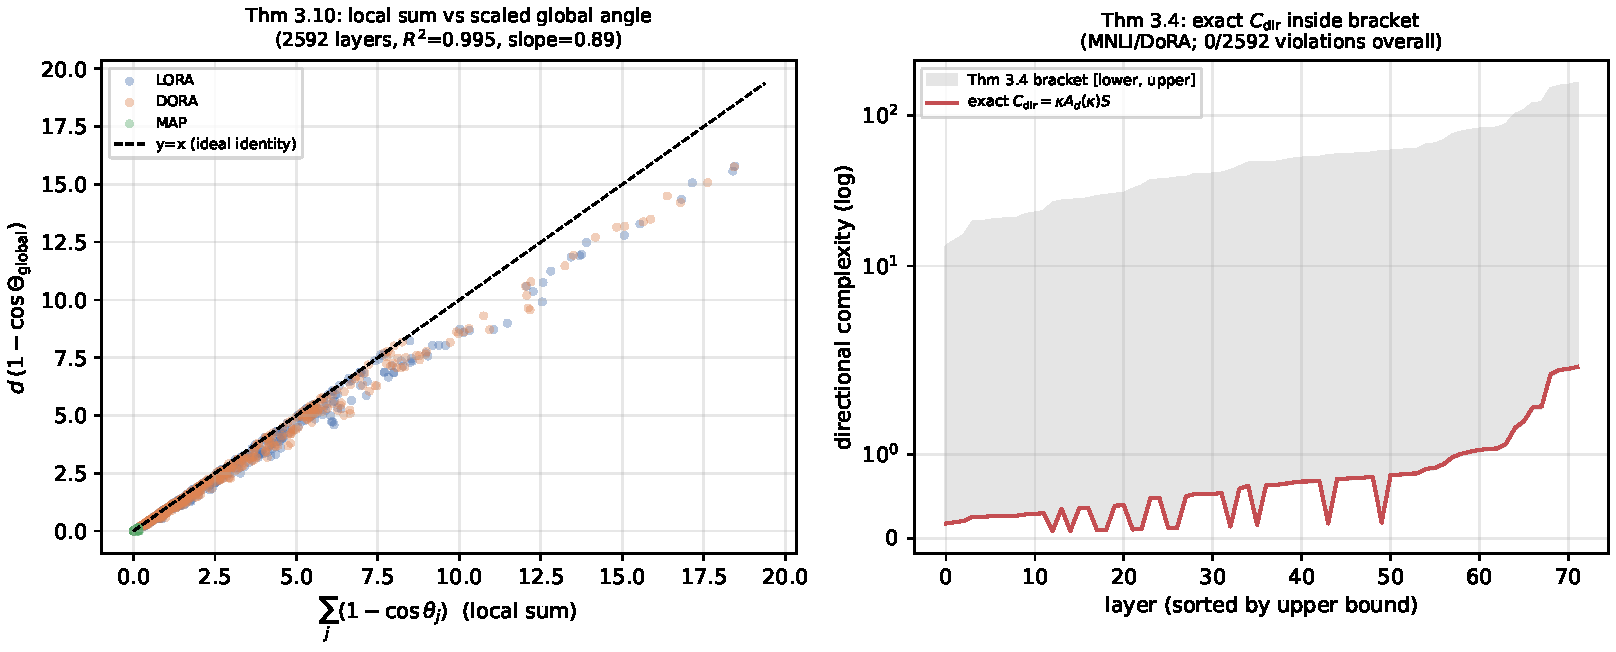
\includegraphics[width=0.95\linewidth]{thm_verify.pdf}
\caption{\textbf{Direct verification on $2592$ measured layers.} (Left)
Theorem~\ref{thm:comparison}: local sum vs.\ dimension-scaled global term, on $y=x$
($R^2{=}0.995$, slope $0.89$). (Right) Theorem~\ref{thm:nonasym}: the exact
$C_{\mathrm{dir}}=\kappa A_d(\kappa)S$ (red) lies inside the analytic bracket (shaded)
for a representative MNLI/DoRA run; $0/2592$ violations overall, hugging the lower
bound because $A_d(\kappa)\ll1$.}
\label{fig:thm}
\end{figure}

\begin{table}[t]
\centering
\caption{Measured directional complexity (summed over $72$ layers, mean over $3$
seeds, $\kappa{=}10$), asymptotic vs.\ non-asymptotic. The $\sim$$10^3$ ratio
$C^{\mathrm{DoRA}}/C^{\mathrm{MAP}}$ is the sum-vs-average gap of
Theorem~\ref{thm:comparison}. QQP and MRPC (below the rule) are the two held-out
tasks, reproducing the same $\sim$$10^3$ ratio.}
\label{tab:cterms}
\small
\begin{tabular}{llcccc}
\toprule
Task & Method & $C^{\mathrm{DoRA}}$ (asym) & $C^{\mathrm{DoRA}}$ (non-asym) & $C^{\mathrm{MAP}}$ & $C^{\mathrm{DoRA}}/C^{\mathrm{MAP}}$ \\
\midrule
SST-2 & LoRA & 498.1  & 5.76  & 0.476 & 1047 \\
      & DoRA & 520.0  & 6.03  & 0.499 & 1043 \\
QNLI  & DoRA & 969.8  & 11.56 & 0.864 & 1122 \\
MNLI  & LoRA & 3837.9 & 45.43 & 3.461 & 1109 \\
      & DoRA & 3902.9 & 46.30 & 3.528 & 1106 \\
RTE   & DoRA & 17.0   & 0.20  & 0.017 & 1008 \\
\midrule
% --- QQP and MRPC: additional held-out tasks (Machine B); verify Thms 3.4 & 3.10 ---
QQP   & LoRA & 2255.7 & 26.83 & 1.838 & 1227 \\
      & DoRA & 2264.3 & 26.93 & 1.846 & 1227 \\
MRPC  & LoRA & 16.8   & 0.20  & 0.017 & 1007 \\
      & DoRA & 17.9   & 0.21  & 0.018 & 1010 \\
\bottomrule
\end{tabular}
\end{table}

\section{Conclusion}
We developed a PAC-Bayesian framework for weight-decomposed PEFT, with non-asymptotic
vMF KL bounds and a comparison theorem characterizing when column-wise (DoRA) vs.\
global (MAP) adaptation is preferable. Empirically, the sum-vs-average identity
(Theorem~\ref{thm:comparison}) and the non-asymptotic KL bracket
(Theorem~\ref{thm:nonasym}) hold on $2592$ measured RoBERTa-base layers, and the
non-asymptotic correction tightens the directional KL by up to $307\times$ at
transformer dimensions---decisive for obtaining meaningful (non-vacuous) bounds.
Extending the directional measurement to a calibrated, magnitude-inclusive estimator
and to domain-shift settings is left to future work.

\appendix
\section{vMF Mean}\label{app:mean}
The vMF partition function is
$Z_d(\kappa)=\int_{\Sd}e^{\kappa\mu^\top x}\,\sigma(dx)=(2\pi)^{d/2}I_{d/2-1}(\kappa)/\kappa^{d/2-1}$.
Differentiating, $\partial_\kappa\ln Z_d(\kappa)=\E_{\vMF(\mu,\kappa)}[\mu^\top x]=A_d(\kappa)$,
confirming $\E[x]=A_d(\kappa)\,\mu$, as used in Lemma~\ref{lem:vmfkl}.

\begin{thebibliography}{9}
\small
\bibitem{dora} S.-Y.\ Liu et al., ``DoRA: Weight-Decomposed Low-Rank Adaptation,''
arXiv:2402.09353, 2024.
\bibitem{map} C.\ Si et al., ``MAP: Revisiting Weight Decomposition for Low-Rank
Adaptation,'' arXiv:2505.23094, 2025.
\bibitem{lora} E.\ J.\ Hu et al., ``LoRA: Low-Rank Adaptation of Large Language
Models,'' arXiv:2106.09685, 2021.
\bibitem{mcallester} D.\ A.\ McAllester, ``Some PAC-Bayesian Theorems,'' \emph{Mach.
Learn.}, 37(3):355--363, 1999.
\bibitem{catoni} O.\ Catoni, \emph{PAC-Bayesian Supervised Classification}, IMS, 2007.
\bibitem{amos} D.\ E.\ Amos, ``Computation of modified Bessel functions and their
ratios,'' \emph{Math.\ Comp.}, 28(125):239--251, 1974.
\bibitem{roberta} Y.\ Liu et al., ``RoBERTa: A Robustly Optimized BERT Pretraining
Approach,'' arXiv:1907.11692, 2019.
\end{thebibliography}

\end{document}
